\documentclass[
    11pt, % Main document font size
    a4paper, % Paper type, use 'letterpaper' for US Letter paper
    oneside, % One page layout (no page indentation)
%twoside, % Two page layout (page indentation for binding and different headers)
    headinclude,footinclude, % Extra spacing for the header and footer
    BCOR5mm, % Binding correction
]{scrartcl}

\usepackage[backend=bibtex,style=vancouver,natbib=true]{biblatex}
\addbibresource{references.bib} % The file with the references

%%%%%%%%%%%%%%%%%%%%%%%%%%%%%%%%%%%%%%%%%
% Arsclassica Article
% Structure Specification File
%
% This file has been downloaded from:
% http://www.LaTeXTemplates.com
%
% Original author:
% Lorenzo Pantieri (http://www.lorenzopantieri.net) with extensive modifications by:
% Vel (vel@latextemplates.com)
%
% License:
% CC BY-NC-SA 3.0 (http://creativecommons.org/licenses/by-nc-sa/3.0/)
%
%%%%%%%%%%%%%%%%%%%%%%%%%%%%%%%%%%%%%%%%%

%----------------------------------------------------------------------------------------
%	REQUIRED PACKAGES
%----------------------------------------------------------------------------------------

\usepackage[
    nochapters, % Turn off chapters since this is an article
    beramono, % Use the Bera Mono font for monospaced text (\texttt)
    eulermath,% Use the Euler font for mathematics
    pdfspacing, % Makes use of pdftex’ letter spacing capabilities via the microtype package
    dottedtoc % Dotted lines leading to the page numbers in the table of contents
]{classicthesis} % The layout is based on the Classic Thesis style

\usepackage{arsclassica} % Modifies the Classic Thesis package


\usepackage[T1]{fontenc} % Use 8-bit encoding that has 256 glyphs

\usepackage[utf8]{inputenc} % Required for including letters with accents

\usepackage{graphicx} % Required for including images
\graphicspath{{Figures/}} % Set the default folder for images

\usepackage{enumitem} % Required for manipulating the whitespace between and within lists

\usepackage{lipsum} % Used for inserting dummy 'Lorem ipsum' text into the template

\usepackage{subfig} % Required for creating figures with multiple parts (subfigures)

\usepackage{amsmath,amssymb,amsthm} % For including math equations, theorems, symbols, etc

\usepackage{varioref} % More descriptive referencing

\RequirePackage{geometry} % Required for adjusting page dimensions and margins

\geometry{
    paper=a4paper, % Paper size, change to letterpaper for US letter size
    top=2.5cm, % Top margin
    bottom=2.5cm, % Bottom margin
    left=2.5cm, % Left margin
    right=2.5cm, % Right margin
    headheight=1cm, % Header height
    footskip=1cm, % Space from the bottom margin to the baseline of the footer
    headsep=1cm, % Space from the top margin to the baseline of the header
}

%----------------------------------------------------------------------------------------
%	THEOREM STYLES
%---------------------------------------------------------------------------------------

\theoremstyle{definition} % Define theorem styles here based on the definition style (used for definitions and examples)
\newtheorem{definition}{Definition}

\theoremstyle{plain} % Define theorem styles here based on the plain style (used for theorems, lemmas, propositions)
\newtheorem{theorem}{Theorem}

\theoremstyle{remark} % Define theorem styles here based on the remark style (used for remarks and notes)

%----------------------------------------------------------------------------------------
%	HYPERLINKS
%---------------------------------------------------------------------------------------

\hypersetup{
%draft, % Uncomment to remove all links (useful for printing in black and white)
    colorlinks=true, breaklinks=true, bookmarks=true,bookmarksnumbered,
    urlcolor=webbrown, linkcolor=RoyalBlue, citecolor=webgreen, % Link colors
    pdftitle={Project Management Group 2 Report}, % PDF title
    pdfauthor={\textcopyright}, % PDF Author
    pdfsubject={}, % PDF Subject
    pdfkeywords={}, % PDF Keywords
    pdfcreator={pdfLaTeX}, % PDF Creator
    pdfproducer={LaTeX with hyperref and ClassicThesis} % PDF producer
}
 % Include the structure.tex file which specified the document structure and layout

\hyphenation{Fortran hy-phen-ation} % Specify custom hyphenation points in words with dashes where you would like hyphenation to occur, or alternatively, don't put any dashes in a word to stop hyphenation altogether

%----------------------------------------------------------------------------------------
%	TITLE AND AUTHOR(S)
%----------------------------------------------------------------------------------------

\title{\normalfont\spacedallcaps{Moderna Vaccine}}

\subtitle{Project Management Coursework}

\author{\spacedlowsmallcaps{Group 2}}

\date{\today} % An optional date to appear under the author(s)

%----------------------------------------------------------------------------------------

\begin{document}

%----------------------------------------------------------------------------------------
%	HEADERS
%----------------------------------------------------------------------------------------

    \renewcommand{\sectionmark}[1]{\markright{\spacedlowsmallcaps{#1}}} % The header for all pages (oneside) or for even pages (twoside)
%\renewcommand{\subsectionmark}[1]{\markright{\thesubsection~#1}} % Uncomment when using the twoside option - this modifies the header on odd pages
    \lehead{\mbox{\llap{\small\thepage\kern1em\color{halfgray} \vline}\color{halfgray}\hspace{0.5em}\rightmark\hfil}} % The header style

    \pagestyle{scrheadings}

%----------------------------------------------------------------------------------------
%	TABLE OF CONTENTS & LISTS OF FIGURES AND TABLES
%----------------------------------------------------------------------------------------

    \maketitle % Print the title

    \setcounter{tocdepth}{2} % Set the depth of the table of contents to show sections and subsections only

    \tableofcontents % Print the table of contents

    \listoffigures % Print the list of figures

    \listoftables % Print the list of tables

%----------------------------------------------------------------------------------------
%	ABSTRACT
%----------------------------------------------------------------------------------------

    \section*{Abstract} % This section will not appear in the table of contents due to the star (\section*)

    \lipsum[1] % Dummy text

    \newpage % Start the article content on the second page, remove this if you have a longer abstract that goes onto the second page
    \section{Introduction}


A statement requiring citation \cite{Figueredo:2009dg}. Reference to Figure~\ref{fig:gallery}.\\

\begin{figure}[tb]
    \centering
    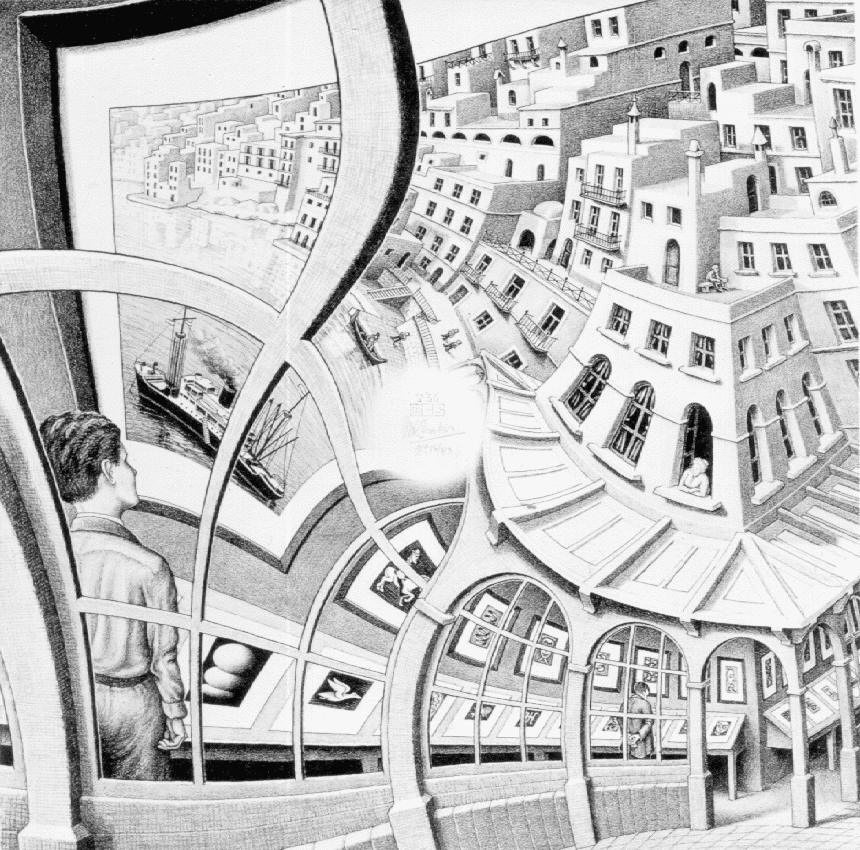
\includegraphics[width=0.5\columnwidth]{GalleriaStampe}
    \caption[An example of a floating figure]{An example of a floating figure (a reproduction from the \emph{Gallery of prints}, M.~Escher,\index{Escher, M.~C.} from \url{http://www.mcescher.com/}).} % The text in the square bracket is the caption for the list of figures while the text in the curly brackets is the figure caption
    \label{fig:gallery}
\end{figure}


\lipsum[1-3] % Dummy text

Some mathematics in the text: $\cos\pi=-1$ and $\alpha$.

    \section{Project Analysis}

\lipsum[5] % Dummy text

\begin{enumerate}[noitemsep] % [noitemsep] removes whitespace between the items for a compact look
    \item First item in a list
    \item Second item in a list
    \item Third item in a list
\end{enumerate}


    \section{Overview}

\subsection{Subsection One!}

\lipsum[6] % Dummy text

\paragraph{Paragraph Description} \lipsum[7] % Dummy text

\subsection{Some Other Subsection}
\paragraph{Different Paragraph Description} \lipsum[8] % Dummy text

    \section{Summary of Lessons}

Some dummy text here
\subsection{Conclusion}

Some smart conclusion here.
Here goes a citation that uses wikipedia and includes a link~\cite{busFactor}.

\begin{itemize}[noitemsep] % [noitemsep] removes whitespace between the items for a compact look
    \item First item in a list
    \item Second item in a list
    \item Third item in a list
\end{itemize}


    \newpage
    \section{Appendix}

\begin{description}
    \item[Word] Definition
    \item[Concept] Explanation
    \item[Idea] Text
\end{description}

\subsection{A Fancy Table}

\begin{table}[hbt]
    \caption{Table of Grades}
    \centering
    \begin{tabular}{llr}
        \toprule
        \multicolumn{2}{c}{Name} \\
        \cmidrule(r){1-2}
        First name & Last Name & Grade \\
        \midrule
        John & Doe & $7.5$ \\
        Richard & Miles & $2$ \\
        \bottomrule
    \end{tabular}
    \label{tab:label}
\end{table}

Reference to Table~\ref{tab:label}. % The \vref command specifies the location of the reference


%----------------------------------------------------------------------------------------
%	BIBLIOGRAPHY
%----------------------------------------------------------------------------------------

    \renewcommand{\refname}{\spacedlowsmallcaps{References}} % For modifying the bibliography heading

%\bibliographystyle{unsrt}
%


    \printbibliography %[heading=bibintoc]

\end{document}
